\documentclass{article}
\usepackage{natbib}
\usepackage[francais]{babel}
\usepackage[utf8]{inputenc}
\usepackage[T1]{fontenc}
\usepackage{hyperref}
\usepackage{graphicx}
\usepackage{minted}
\usepackage{uqac}

% ================================ Meta data (pour titre et autre)
\discipline{8INF844}
\supervisor{Abdenour Bouzouane}
\project{Projet}
\title{Bearer Assistant}
\author{Sébastien Blin\\Victor Drouin Viallard}

% ================================ Document
\begin{document}

\maketitle

\section{Description}
TODO décrire ce qu'on souhaite mettre en place


\section{Installation}
\subsection{Choregraphe}

Choregraphe est une suite logicielle qui facilite les interactions avec NAOqi (la bibliothèque utilisée pour programmer le Nao en C++ ou Python). On peut l'utiliser pour créer des animations ou des comprotements, tester ces comportements sur des robots simulés ou réels, et obtenir un retour des composants du Nao tel que les deux caméras. On peut décrire les comportements à l'aide de boites (programmation graphique) ou en créant nos propres boites en Python. L'interaction avec NAOqi est simplifiée, mais l'exécution sera plus lente qu'un script Python ou un code C++. [Fig \ref{fig:choregraphe}]

\begin{figure}[h]
	\begin{center}
			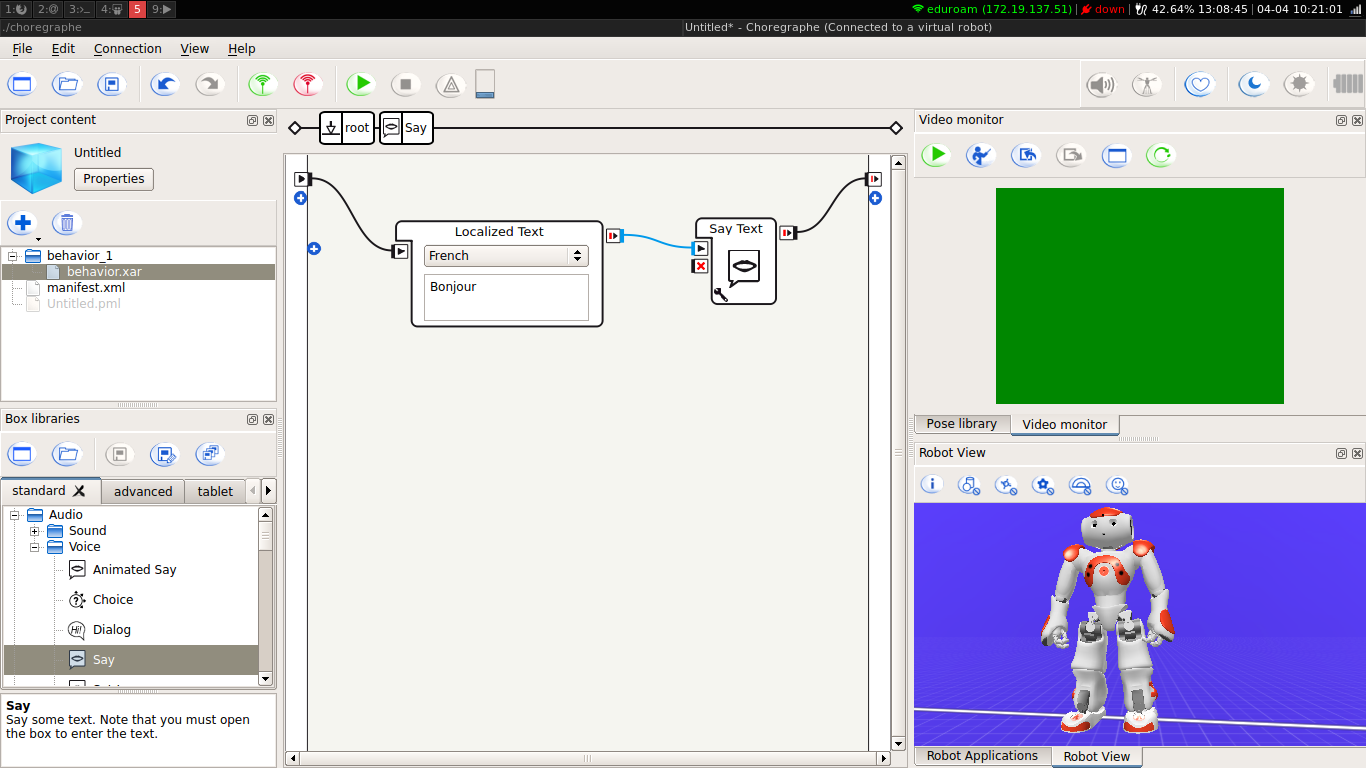
\includegraphics[scale=0.2]{img/choregraphe}
		\caption{Choregraphe}
		\label{fig:choregraphe}
	\end{center}
\end{figure}

Pour l'installer il suffit de se rendre sur la page~: \url{https://developer.softbankrobotics.com/us-en/downloads/nao-v5-v4} et de prendre le lien \emph{Choregraphe VERSION PLATFORM Binaries} qui contiendra l'application ainsi que les bibliothèques utiles dans la section suivante.

\subsection{Environnement Python}

Nous avons choisi de ne pas utiliser Choregraphe pour la programmation du robot (pour des raisons de flexibilité, de performances) mais de le contrôler avec Python (version 2, les bibliothèques n'étant pas encore compatible Python 3). Une fois que choregaphe a bien été installé, il suffit de se rendre dans le dossier \emph{/lib} du dossier téléchargé pour obtenir les librairies utilisées en Python et C++. Il suffit alors de copier les librairies que vous souhaitez avec votre projet afin de pouvoir utiliser NAOqi.
Pour tester, vous pouvez vous rendre dans le dossier où se trouve ces bibliothèques~:
\begin{minted}{python}
  AmarOk@tars2 ~ : cd Downloads/choregraphe-suite-2.1.4.13-linux64/lib
  AmarOk@tars2 ~/Downloads/choregraphe-suite-2.1.4.13-linux64/lib : python
 Python 2.7.13 (default, Jan 12 2017, 17:59:37)
 [GCC 6.3.1 20161221 (Red Hat 6.3.1-1)] on linux2
 Type "help", "copyright", "credits" or "license" for more information.
 >>> import naoqi
 >>> # Ici vous pouvez utiliser NAOqi
\end{minted}

\subsection{Connexion au robot Nao}

Une fois les outils installés, il est possible de se connecter au Nao afin de le controler.
La première étape est d'allumer le Nao en le reliant en lien direct à votre PC ou en le connectant au WiFi (s'il est configuré pour se rendre sur un réseau WiFi).

\subsubsection{En lien direct depuis linux}

Il suffit de créer un réseau local avec le Nao. Il existe énormément de moyens de configurer ce réseau. Un des outils possible est de configurer une telle connexion est \emph{nm-connection-editor}. Pour se faire, il suffit d'ouvrir \emph{nm-connection-editor}, d'éditer la connexion ethernet et dans l'onglet \emph{IPv4 Settings}, configurer le type de connexion en \emph{Local-link only}

\begin{figure}[h]
	\begin{center}
			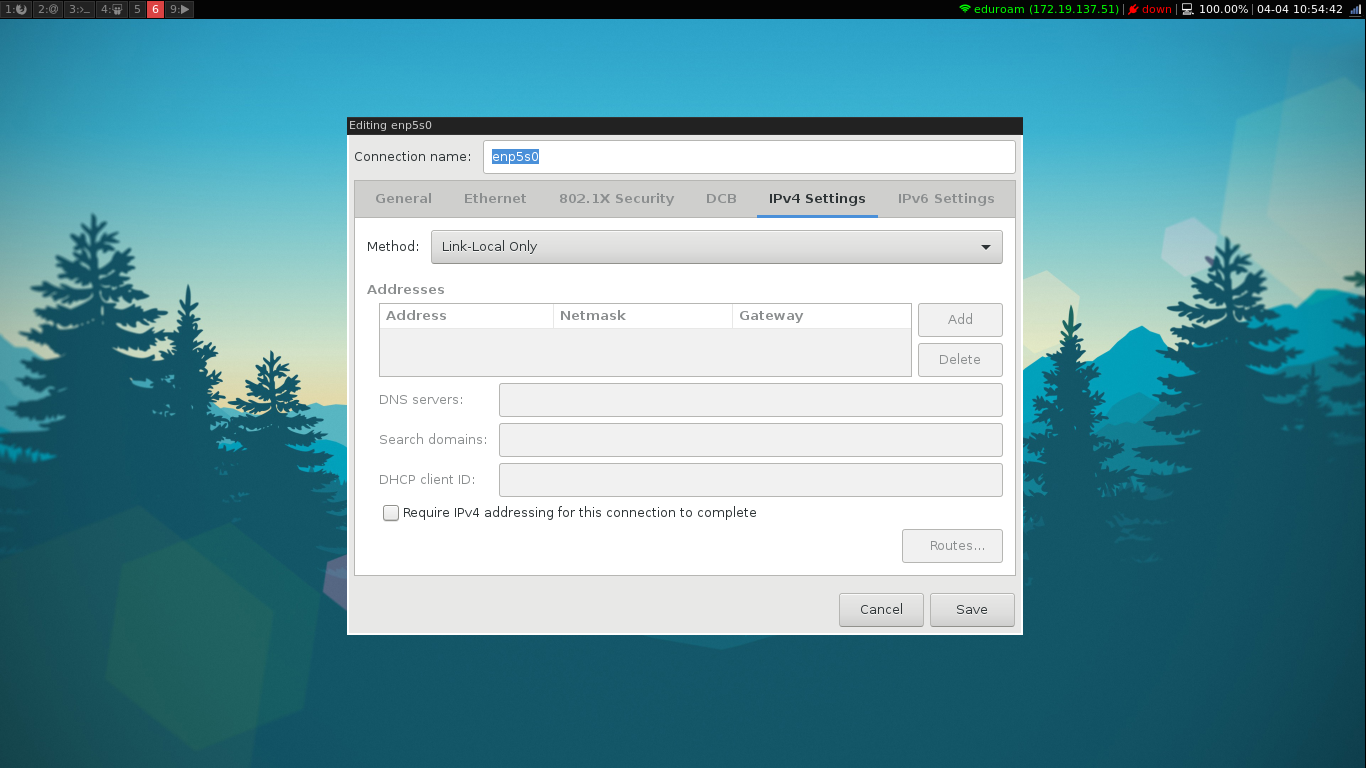
\includegraphics[scale=0.2]{img/nm-connection-editor}
		\caption{nm-connection-editor}
		\label{fig:nm-connection-editor}
	\end{center}
\end{figure}

Après 1 ou 2 minutes, le Nao aura une adresse ip accessible, vous pourrez alors le configurer depuis l'interface du robot (\emph{login: nao, password: nao}). Il sera par exemple possible dans l'onglet connectivité de configurer le Nao pour rejoindre un réseau WiFi.

\subsubsection{En lien direct depuis windows}

TODO

\subsubsection{Via WiFi}

Si le robot a été configuré pour rejoindre un réseau WiFi, il s'y connectera automatiquement et récupérera une IP.

\section{Programmation via Python 2}

\subsection{NAOqi}

\subsubsection{Le broker}

Normalement, le broker est géré de manière transparente. On en a seulement besoin si on souhaite réaliser des modules qui réagissent à un évènement via un callback. Le processus est documenté ici~: \url{http://bx.psu.edu/~thanh/naoqi/dev/python/reacting_to_events.html#python-reacting-to-events}.

\subsubsection{Les proxies}

Un proxy se comporte comme le module qu'il décrit. Par exemple si on utilise un proxy vers \emph{ALTextToSpeech} on aura accès aux méthodes de ce module (comme \emph{say()} par exemple).

\subsection{Les différents modules}

\subsubsection{Synthèse vocale\footnote{\url{http://doc.aldebaran.com/1-14/naoqi/audio/altexttospeech-api.html#altexttospeech-api}}}

Pour utiliser la synthèse vocale du Nao, il suffit de créer un proxy pour \emph{ALTextToSpeech}~:

\begin{minted}{python}
  from naoqi import ALProxy
  tts = ALProxy('ALTextToSpeech', IP_NAO, PORT_NAO)
  tts.setLanguage('French')
  tts.say('bonjour')
\end{minted}

\subsubsection{Reconnaissance des visages}

La reconnaissance des visages se fait à l'aide du proxy \emph{ALFaceDetection} qui se charge d'écrire dans la mémoire s'il détecte un visage. Voici un code de base~:

\begin{minted}{python}
  from naoqi import ALProxy
  import time

  face_proxy = ALProxy('ALFaceDetection', IP_NAO, PORT_NAO)
  memory = ALProxy('ALMemory', IP_NAO, PORT_NAO)
  time.sleep(1)
  val = self.memory.getData('FaceDetected')
  print(val) # Donne les informations des visages détectés
\end{minted}

La documentation de l'API est disponible ici~:
\url{http://doc.aldebaran.com/1-14/naoqi/vision/alfacedetection-api.html#alfacedetection-api}

\subsubsection{Apprentissage et reconnaissance d'objets}

Une des méthodes pour utiliser la reconnaissance d'objets du Nao est d'utiliser \emph{Choregraphe} (la seconde est d'utiliser une application externe travaillant sur le flux de la caméra, mais ne sera pas détaillée ici).
La documentation se trouve à cette adresse url~: \url{http://doc.aldebaran.com/1-14/software/choregraphe/tutos/recognize_objects.html} et peut-être utilisé avec \emph{Python} avec le code détaillé ici~: \url{http://doc.aldebaran.com/1-14/naoqi/vision/alvisionrecognition-tuto.html#alvisionrecognition-tuto}

\subsubsection{Reconnaissance vocale}
Une autre possibilité que nous pouvons mettre en place est de réagir aux évènements. Par exemple, pour la reconnaissance vocale, il est possible de réaliser un module qui réagit à la reconnaissance d'un mot. Il est possible de réaliser un module de ce type (et ainsi éviter le fait de devoir écouter pendant quelques secondes et de regarder si un mot a été reconnu) à l'aide d'un broker personnalisé~:

\begin{minted}{python}
from naoqi import ALProxy
from naoqi import ALBroker
from naoqi import ALModule

AgentNao = None

class Module(ALModule):
    def __init__(self, name):
        ALModule.__init__(self, name)
        self.memory = ALProxy('ALMemory')
        self.speech_recognition = ALProxy('ALSpeechRecognition')
        self.speech_recognition.setLanguage('French')

    def detect_word(self, vocabulary):
        try:
            self.memory.unsubscribeToEvent('WordRecognized', 'AgentNao')
        except:
            pass
        self.speech_recognition.setVocabulary(vocabulary, False)
        self.memory.subscribeToEvent('WordRecognized', 'AgentNao',
                                     'onWordRecognized')

    def onWordRecognized(self, key, value, message):
        self.memory.unsubscribeToEvent('WordRecognized', 'AgentNao')
        print('Recognized')
        print(key)
        print(value)
        print(message)

if __name__ == '__main__':
    broker = ALBroker('broker', '0.0.0.0', 0, NAO_IP, NAO_PORT)

    global AgentNao
    AgentNao = Module('AgentNao')
    vocabulary = ['oui', 'non', 'yes', 'no']
    words_recognized = AgentNao.detect_word(vocabulary)
    try:
        while True:
            time.sleep(1)
    except KeyboardInterrupt:
        print('Interrupted by user, shutting down')
        broker.shutdown()
        sys.exit(0)
\end{minted}



La documentation de l'API de cette partie est disponible ici~: \url{http://doc.aldebaran.com/2-1/naoqi/audio/alspeechrecognition-api.html#alspeechrecognition-api}


\subsubsection{Postures}

Ce module est utilisé pour mettre le Nao dans une position prédéfinie (comme debout, assis, etc). Les différentes postures sont disponibles ici \url{http://doc.aldebaran.com/2-1/family/robots/postures_robot.html} et la documentation ici \url{http://doc.aldebaran.com/1-14/naoqi/motion/alrobotposture-api.html}

\begin{minted}{python}
  from naoqi import ALProxy
  posture_proxy = ALProxy('ALRobotPosture', IP_NAO, PORT_NAO)
  posture_proxy.goToPosture('StandInit', 0.5)
\end{minted}

\subsubsection{Mouvement}
Il existe de nombreuses fonctions de faire bouger le robot. La documentation se trouve ici~: \url{http://doc.aldebaran.com/2-1/naoqi/motion/almotion-api.html}

Voici quelques exempless de code pour mouvoir le Nao. Tout d'abord, pour le faire avancer~:
\begin{minted}{python}
from naoqi import ALProxy
from naoqi import ALBroker
from naoqi import ALModule
import math

motion_proxy = ALProxy('ALMotion', IP_NAO, PORT_NAO)
motion_proxy.wakeUp()
# Le faire faire demi-tour
motion_proxy.moveTo(0, 0, math.pi)
# Le faire avancer tout droit
motion_proxy.moveTo(0.2, 0, 0)
\end{minted}

Il est aussi possible de contrôler les bras, par exemple faire tendre le bras au robot. Cette partie est plus complexe à prendre en main car il faut manipuler un objet Position6D. La documentation se trouve ici~: \url{http://doc.aldebaran.com/2-1/naoqi/motion/control-cartesian.html#control-cartesian}
\begin{minted}{python}
from naoqi import ALProxy
from naoqi import ALBroker
from naoqi import ALModule
import almath
import math
import motion

motion_proxy = ALProxy('ALMotion', IP_NAO, PORT_NAO)
motion_proxy.wakeUp()
motion_proxy.wakeUp()

effector = 'RArm'
space = motion.FRAME_ROBOT
axisMask = almath.AXIS_MASK_VEL    # just control position
isAbsolute = False

# Since we are in relative, the current position is zero
currentPos = [0.0, 0.0, 0.0, 0.0, 0.0, 0.0]

# Define the changes relative to the current position
dx = 0.1      # translation axis X (meters)
dy = 0.0      # translation axis Y (meters)
dz = 0.12      # translation axis Z (meters)
dwx = 0.00      # rotation axis X (radians)
dwy = 0.00      # rotation axis Y (radians)
dwz = 0.00      # rotation axis Z (radians)
targetPos = [dx, dy, dz, dwx, dwy, dwz]
# Go to the target
path = [currentPos, targetPos]
times = [2.0, 4.0]

motion_proxy.positionInterpolation(effector, space, path,
axisMask, times, isAbsolute)
motion_proxy.openHand('RHand')
\end{minted}

Enfin, il est possible de réaliser un module réagissant à une pression sur un des multiples capteurs\footnote{\url{http://doc.aldebaran.com/2-1/family/robots/contact-sensors_robot.html#robot-contact-sensors}}. Par exemple~:

\begin{minted}{python}
from naoqi import ALProxy
from naoqi import ALBroker
from naoqi import ALModule

AgentNao = None

class Module(ALModule):
    def __init__(self, name):
        ALModule.__init__(self, name)
        self.memory = ALProxy('ALMemory')
        self.memory.subscribeToEvent('TouchChanged', 'AgentNao', 'onTouched')

    def onTouched(self, strVarName, value):
        ''' This will be called each time a touch
        is detected.

        '''
        # Unsubscribe to the event when talking,
        # to avoid repetitions
        self.memory.unsubscribeToEvent('TouchChanged', 'AgentNao')

        touched_bodies = []
        for p in value:
            if p[1]:
                print(p[0])

        self.close_hand(touched_bodies)

        # Subscribe again to the event
        self.memory.subscribeToEvent('TouchChanged', 'AgentNao', 'onTouched')

if __name__ == '__main__':
    broker = ALBroker('broker', '0.0.0.0', 0, NAO_IP, NAO_PORT)

    global AgentNao
    AgentNao = Module('AgentNao')
    vocabulary = ['oui', 'non', 'yes', 'no']
    words_recognized = AgentNao.detect_word(vocabulary)
    try:
        while True:
            time.sleep(1)
    except KeyboardInterrupt:
        print('Interrupted by user, shutting down')
        broker.shutdown()
        sys.exit(0)
\end{minted}


\section{BearerAssistant}

\subsection{Description}

Le sujet de notre projet a été modifié au fur et à mesure de la découverte des APIs du Nao et du temps disponible. Au début, nous souhaitions réaliser un robot assistant qui traduisait une commande en langage des signes. Au final, nous nous sommes orientés vers un robot qui se charge de demander à une personne s'il peut prendre un objet et de l'apporter à une autre personne. Au départ, il se trouve dans une position assise. Il se lève dès qu'il détecte une personne, lui demande s'il peut prendre un objet. Si la personne répond oui, le Nao tend le bras (sinon il retourne au départ) et attend un objet. Une personne lui donne alors l'objet, appuie sur le capteur à l'arrière de la main. Le nao sert sa main, baisse son bras et se retourne. Il cherche alors une nouvelle personne, va vers cette personne et lui lache l'objet. Enfin, il retourne à sa position et se rasseoit.

TODO, dire ce que fait le robot (ou ce qu'on voulait qu'il fasse)
\subsection{Architecture du code}
TODO, expliquer l'architecture du code et pourquoi c'est agent
\subsection{Ce qui a été réalisé}
TODO, fonctionnalité
\subsection{Pistes d'amélioration}
TODO (comment améliorer le Nao, ce qui n'a pas été fait)

\end{document}
